\section{Theory}
\label{sec:theory}

THIS SECTION IS JUST COPYPASTED STUFF NOW. DON'T EXPECT IT TO FIT WITH THE REST OF THE PAPER

\newtheorem{problem}{Problem}

\newcommand{\bigo}{\mathcal{O}}
\newcommand{\page}{\pi}
\newcommand{\str}{s}
\newcommand{\node}{\mathcal {n}}
\newcommand{\W}{\mathcal {W}}

\subsection{Defining the problem formally}
Given that all pages have the same length, and that all objects are of the same size, we may represent pages as binary strings of length $b$ equal to the maximum number of objects that the page can store. We represent each page $\page$ with string $\str$ such that $\str(i) = 1$ if $\page$ has an object at offset $i$, and 0 otherwise.

\begin{definition}
We say that two binary strings $\str_{1}, \str_{2}$ \textbf{mesh}  iff $\str_{1}(i) + \str_{2}(i) \leq 1$ $\forall i \in [0,b-1]$.\\
We say that k binary strings $\str_{1}, ... \str_{k}$ mesh iff $\sum_{j \in [1,k]} \str_{j}(i) \leq 1$ $\forall i \in [0,b-1]$.\\
Equivalently, k binary strings mesh if each each of said strings are pairwise meshable with all of the other strings.
\end{definition}

We would like to develop an algorithm to optimally mesh any multi-set of strings.  But what exactly does it mean to mesh optimally?  When we mesh k pages together, all of the objects scattered around those k pages are moved to a single page; the remaining k-1 pages become empty and can be released to the operating system.  So we can say that we "release" k-1 strings when we mesh k strings together.  Since our goal is to completely empty as many physical pages as possible, we can characterize our theoretical problem as:

\begin{problem}
Given a multi-set of $m$ binary strings of length $b$, find a meshing that will release the maximum number of strings.
\end{problem}

Note that the total number of strings released is equal to $m - \rho - \phi$ where $\rho$ is the number of total meshes performed and $\phi$ is the number of strings that remain unmeshed.

\subsection{Graph Interpretation}
This meshing problem is reducible to min clique cover.  We implictly show this reduction through a straightforward graph interpretation of the meshing problem, and then argue that for most practical cases there will be few triangles in the meshing graph, implying that we can consider the maximum matching problem on this graph instead of clique cover.
\subsubsection{Definition}
Given a string multi-set $S$, we construct a meshing graph $G_S$ as follows:\\
We add a node $\node$ to $G_S$ for each $\str \in S$.  We say node $\node$ represents $\str$.  For each node pair $\node_1, \node_2$, we add edge $(\node_1, \node_2)$ iff $\node_1$ and $\node_2$ mesh.

\begin{figure}[h]
\includegraphics[scale = 0.5]{figures/graph_interpretation.png}
\centering
\caption{The meshing graph generated from string set \{110100, 101000, 010011, 001000\}.}
\end{figure}

If a subset of the strings in $S$ are meshable, the corresponding set of nodes in the meshing graph form a clique.  If we choose some clique cover on the graph, this is equivalent to a legal meshing of strings in the string multi-set (where trivial cliques of size one represent unmeshed strings).  The number of cliques is exactly equal to the corresponding number of meshes and unmeshed nodes, which is precisely the quantity we are trying to minimize.


Note that while we have shown that the meshing problem is reducible to min clique cover, we have not shown that the meshing problem is NP-Hard.  The meshing problem is indeed NP-hard for strings of arbitrary length, but in all practical cases string length is a constant.  

\begin{theorem}
The meshing problem for $S$, a multi-set of strings of constant length is in P; equivalently, the min clique cover problem on meshing graphs generated from sets of strings of constant length is in P.
\end{theorem}
\begin{proof}
We assume without loss of generality that $S$ does not contain the all-zero string $\str_0$; if it does, since $\str_0$ can be meshed with any other string and thus can always be released, we can solve the meshing problem for $S \setminus \str_0$ and then mesh each instance of $\str_0$ arbitrarily.

Rather than reason directly about the min clique cover problem on some bounded-length meshing graph $G$, let us consider the equivalent problem of coloring $\bar{G}$, the complement of $G$.  $\bar{G}$ has an edge between  every pair of two nodes whose strings do not mesh.

$\bar{G}$'s node set N can be partitioned into at most $2^b-1$ subsets $N_1, N_2, ... N_{2^b-1}$ such that all nodes in $N_i$ represent the same string $\str_i$ $\forall i$.  The induced subgraph of $N_i$ is a clique since all its nodes have a 1 in the same position and thus cannot be pairwise meshed.  Further, all nodes in $N_i$ has the same neighbors since they all represent the same string.

Since $N_i$ is a clique, at most one node in $N_i$ may be colored with any color.  Fix some coloring on $\bar{G}$.  Swapping the colors of two nodes in $N_i$ does not change the validity of the coloring since these nodes have the same neighbor set.  Thus, we can unambiguously represent a valid coloring of $\bar{G}$ merely by indicating in which cliques each color appears.
PROOF UNFINISHED WRITE UP COUNTING PART
- there are at most v plus one to the 2 to the 2 to the b of these partitions, polynomial
- just try em all
\end{proof}

\subsubsection{Random Properties}
For all real-world instances of the meshing problem we expect to solve, the string set is produced randomly (due to our assumptions about memory operations).  Thus the interpretation described above defines a new variety of random graph.  Depending on the distribution on strings in the string set, we can identify some properties of the random graph.

\subsubsection{Case 1: Constant occupancy}
Assume that each string in $S$ has exactly $n$ ones.  In other words, each string has occupancy $n$.  Then the probability of an edge in the meshing graph is $q = \frac{{{b-n}\choose{n}}}{{{b}\choose{n}}}$.  The degree of each node is \texttildelow $Bin(m-1,q)$.  While edges are two-way independent, they are not necessarily three-way independent - specifically, possible edges in a cycle are not independent of each other.

\subsubsection{Case 2: Independent bits}
Assume that each bit in each string is 1 independently with probability p.  Then the occupancy of each string is a random variable $n$ \texttildelow $Bin(b, p)$ with mean $bp$.  The probability of an edge in the meshing graph is $q = (1-p^2)^n$.  Unlike the constant 
occupancy case, we cannot even say that edges are two-way independent - possible edges connected by any path are not independent of each other.

\subsection{Clique Cover and Max Matching}
Minimum Clique Cover is NP-Hard, suggesting that finding fast, optimal algorithms for computing meshing may not be a reasonable goal.  Worse, Zuckerman \cite{zuckerman07} shows that approximation of min clique cover to within a $m^{1-\epsilon}$ factor of optimal is also NP-hard.

Luckily, approximating the min clique cover may not be necessary, even if we desire near-optimal meshings - we can simply compute the maximum matching (a much easier computational task) instead.  This is because triangles (and therefore larger cliques) are rare in meshing graphs.  In a graph with no triangles, the min clique cover problem degenerates to the maximum matching problem.  In a graph with few triangles (and therefore no larger cliques whp), the min clique cover will differ by the maximum matching by at most 1 for every triangle.\\

Intuitively, an edge in a meshing graph can be thought of as an indicator of \textit{difference} between two strings.  If strings $\str_1$ and $\str_2$ mesh, and $\str_2$ and $\str_3$ mesh, then $\str_1$ and $\str_3$ are both different from $\str_2$, which means they are more likely to be the same (and thus not mesh).

More rigorously, in the constant occupancy case, the probability of a triangle between any three nodes is $$\frac{{{b-n}\choose{n}}}{{{b}\choose{n}}}\frac{{{b-2n}\choose{n}}}{{{b}\choose{n}}}$$ so the expected number of triangles in the entire graph is $${{m}\choose{3}}\frac{{{b-n}\choose{n}}}{{{b}\choose{n}}}\frac{{{b-2n}\choose{n}}}{{{b}\choose{n}}}$$.

In most practical cases, we will not be interested in meshing strings with low occupancy - it is often better just to wait until the last objects on these pages are freed.  For higher occupancies, the expected number of triangles is quite low.  For instance, if $b = 32, n = 10, m = 1000$, we expect to have less than two triangles in the meshing graph.

We experimentally verify this result by generating many random constant occupancy graphs and, for each graph, comparing the size of the maximum matching to the size of a greedy (non-optimal) solution for min clique cover.  The results are summarized in the figure below.

\begin{figure}[h]
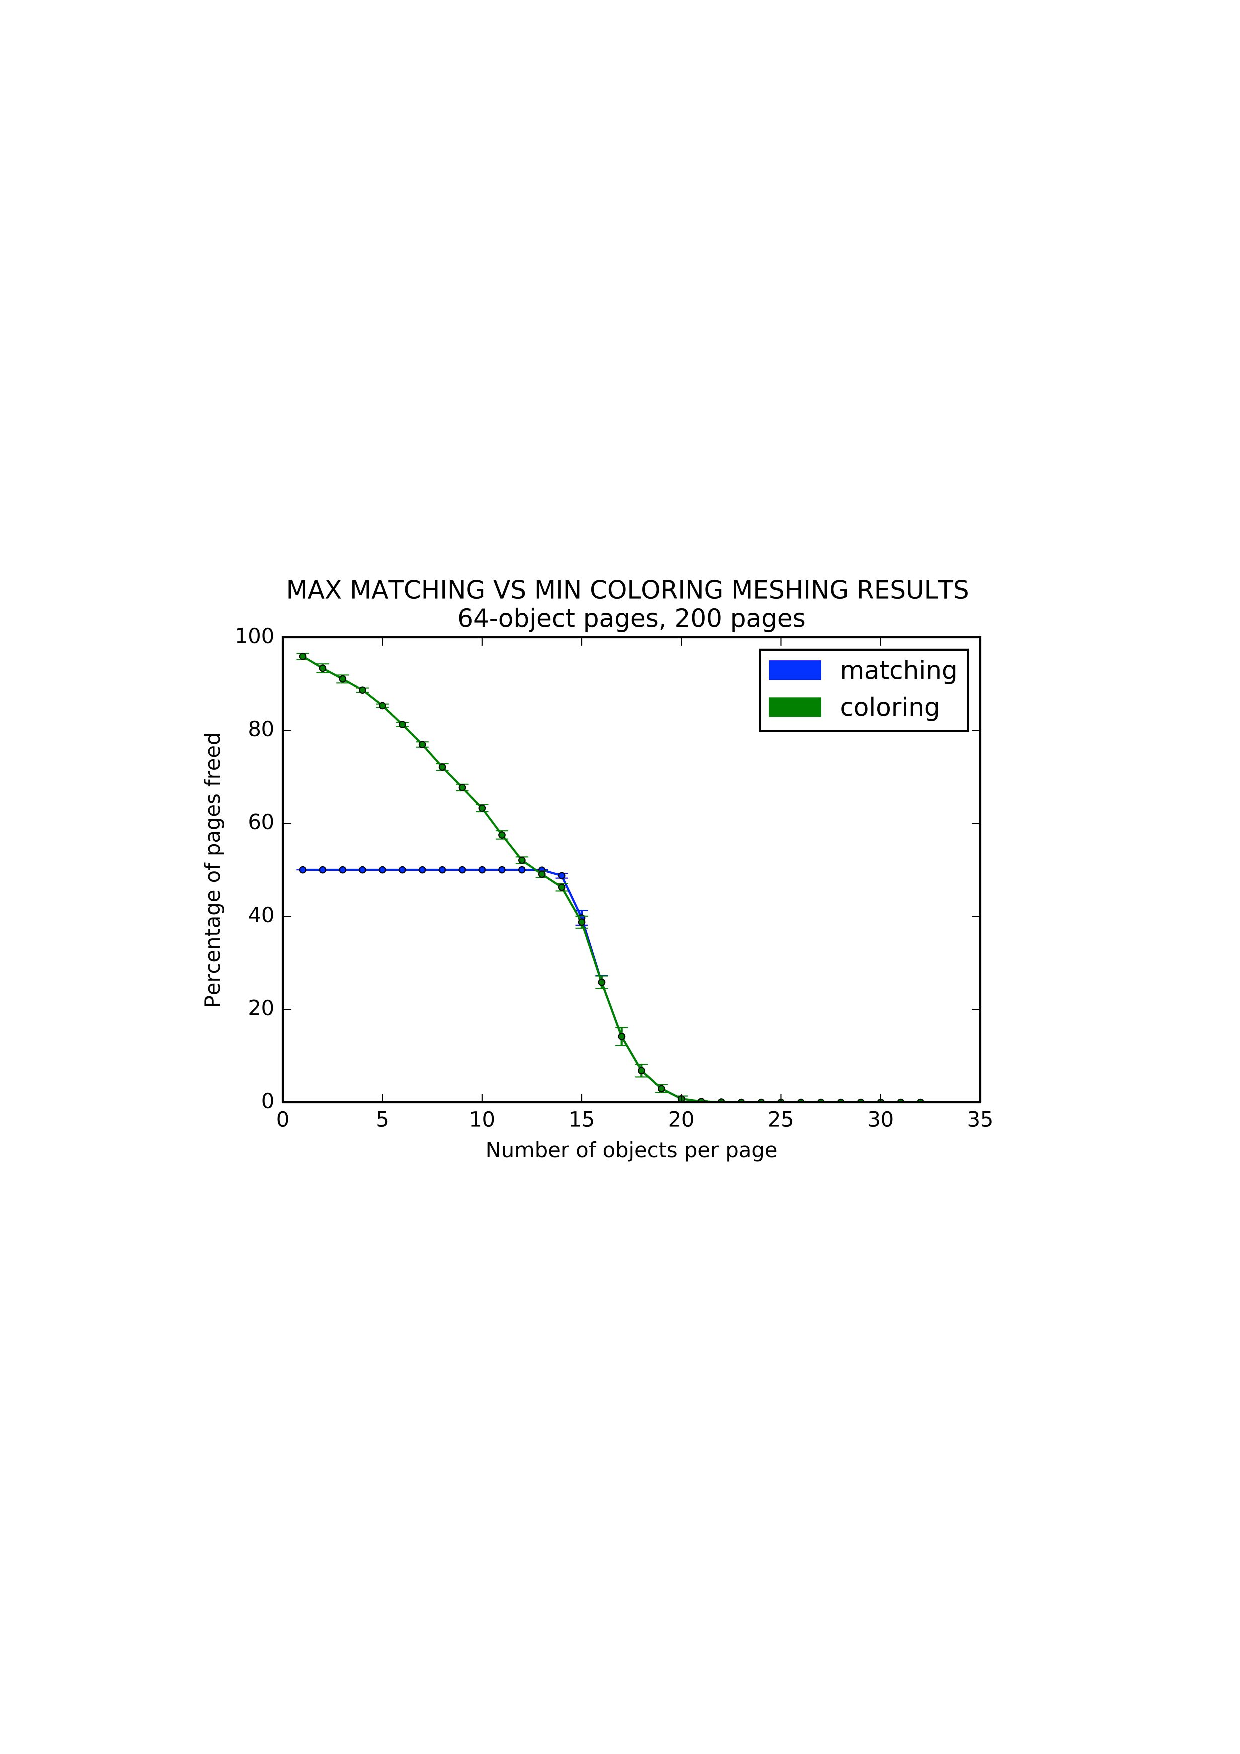
\includegraphics[scale = .5]{figures/comparison.pdf}
\centering
\caption{Average values for max matching and min clique cover on randomly generated graphs.  Ten graphs were generated for each occupancy.}
\end{figure}

For these parameters the $n = 10$ to $n = 17$ range is where we are most likely to try meshing.  See the "Thresholds" section below for more detail on how this is determined.\\

For independent bit graphs, the probability that any three nodes form a clique is $$((1-p)^3 - 3(1-p)^2p)^b$$ so the expected number of triangles for the entire graph is $${{m}\choose{3}}((1-p)^3 - 3(1-p)^2p)^b$$.

This is signficantly larger than the constant occupancy case for similar expected occupancy.  For $p = \frac{n}{b} = \frac{10}{32}, m = 1000$, the expected number of triangles is roughly 36,000.  However, we can see experimentally that these graphs behave quite similarly:


\begin{figure}[h]
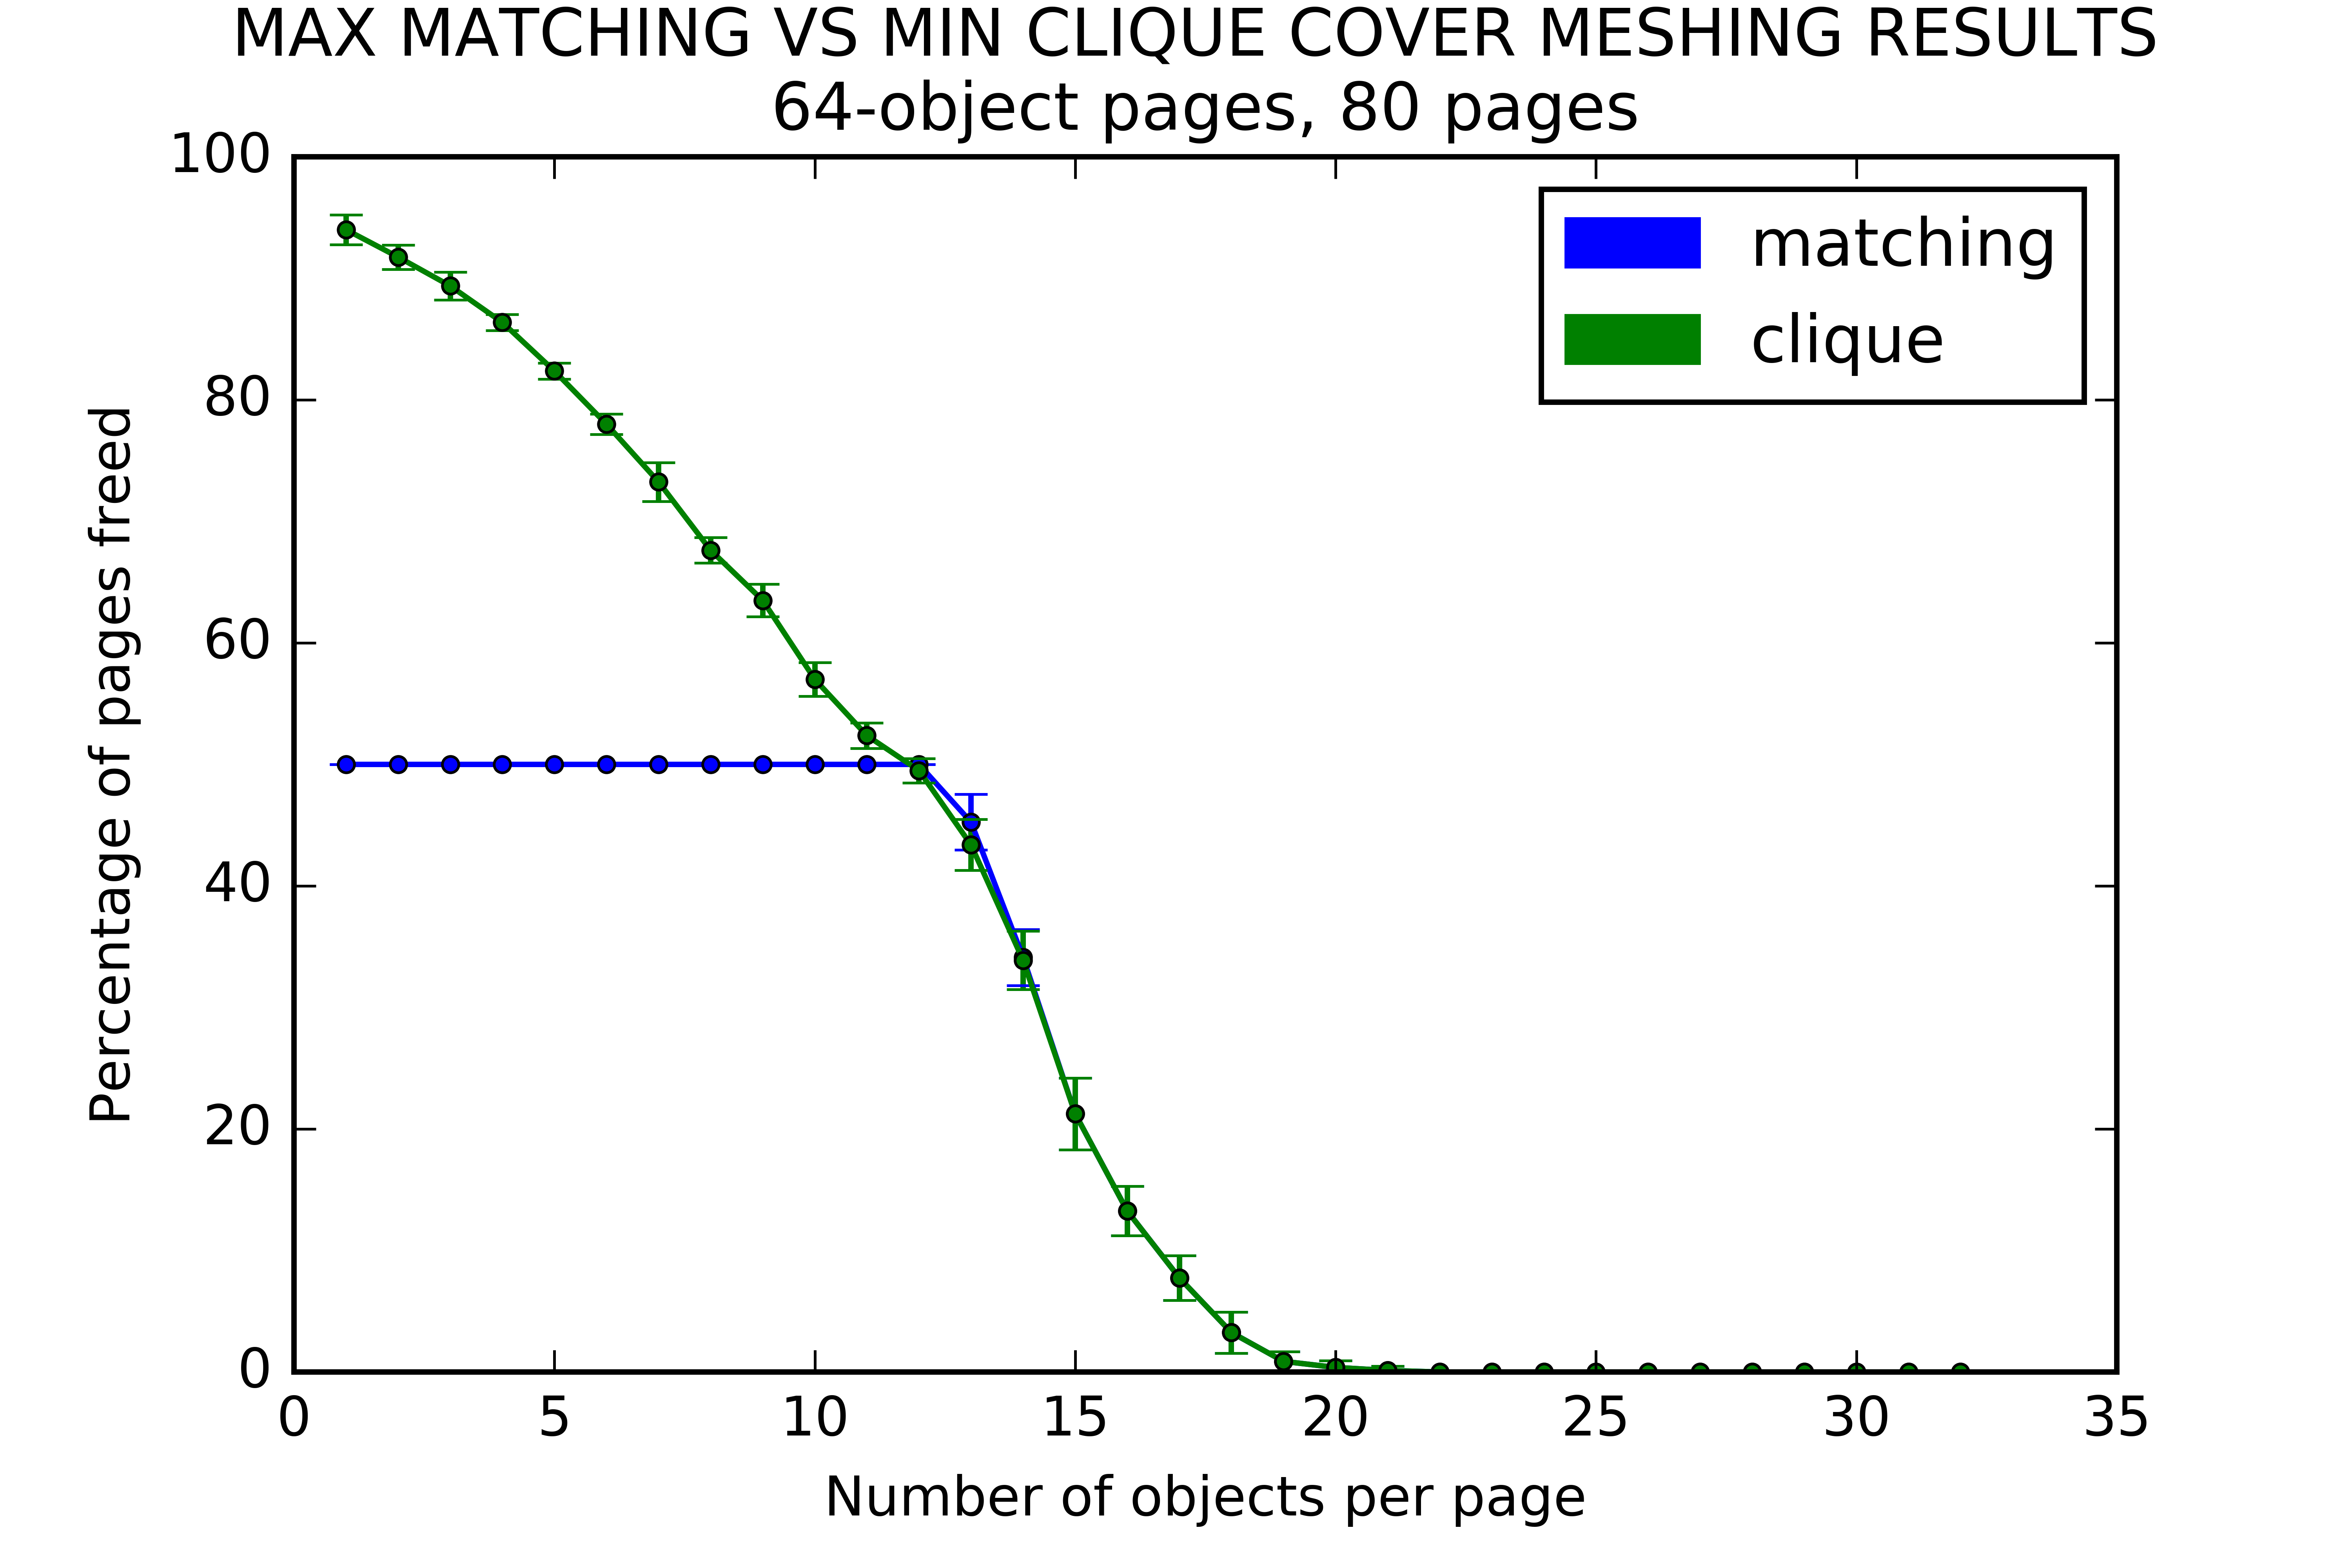
\includegraphics[scale = .5]{figures/64m80ind.png}
\centering
\caption{Average values for max matching and min clique cover on randomly generated graphs.  Graphs were generated from string sets according to the independent bits model; $p = \frac{n}{b}$.  Ten graphs were generated for each occupancy.}
\end{figure}

While constant occupancy graphs are fairly regular, independent bit graphs may not be - since strings have different occupancies, nodes which correspond to strings with relatively low occupancy will tend to have significantly higher degree than other nodes in the graph.  Meanwhile, other nodes may have strings with high occupancy, and therefore only have a few edges (probably with low-occupancy nodes).  So while there are many triangles, when the graph is sparse enough, even meshing cliques of size 3 and 4 will likely "abandon" adjacent high-occupancy nodes, one of which could have been matched with the high degree node to yield the same number of releases.\\

So in this case we still expect finding the maximum matching to be good enough.

\subsection{Experimental Comparison}
We might wonder how the maximum matching varies between our two types of random graphs (constant occupancy and independent bits).  To this end, we randomly generated many graphs using both frameworks and determined the size of their maximum matchings.  A summary of the results is displayed below.  Constant occupancy graphs were created by randomly generating strings sets by drawing each string uniformly at random from the set of all length 80 with occupancy $n$.  Independent bit graphs were created by randomly generating string sets by choosing $p$ such that the expected occupancy for each string is equal to $n$, so that the two can be meaningfully compared.


\begin{figure}[h]
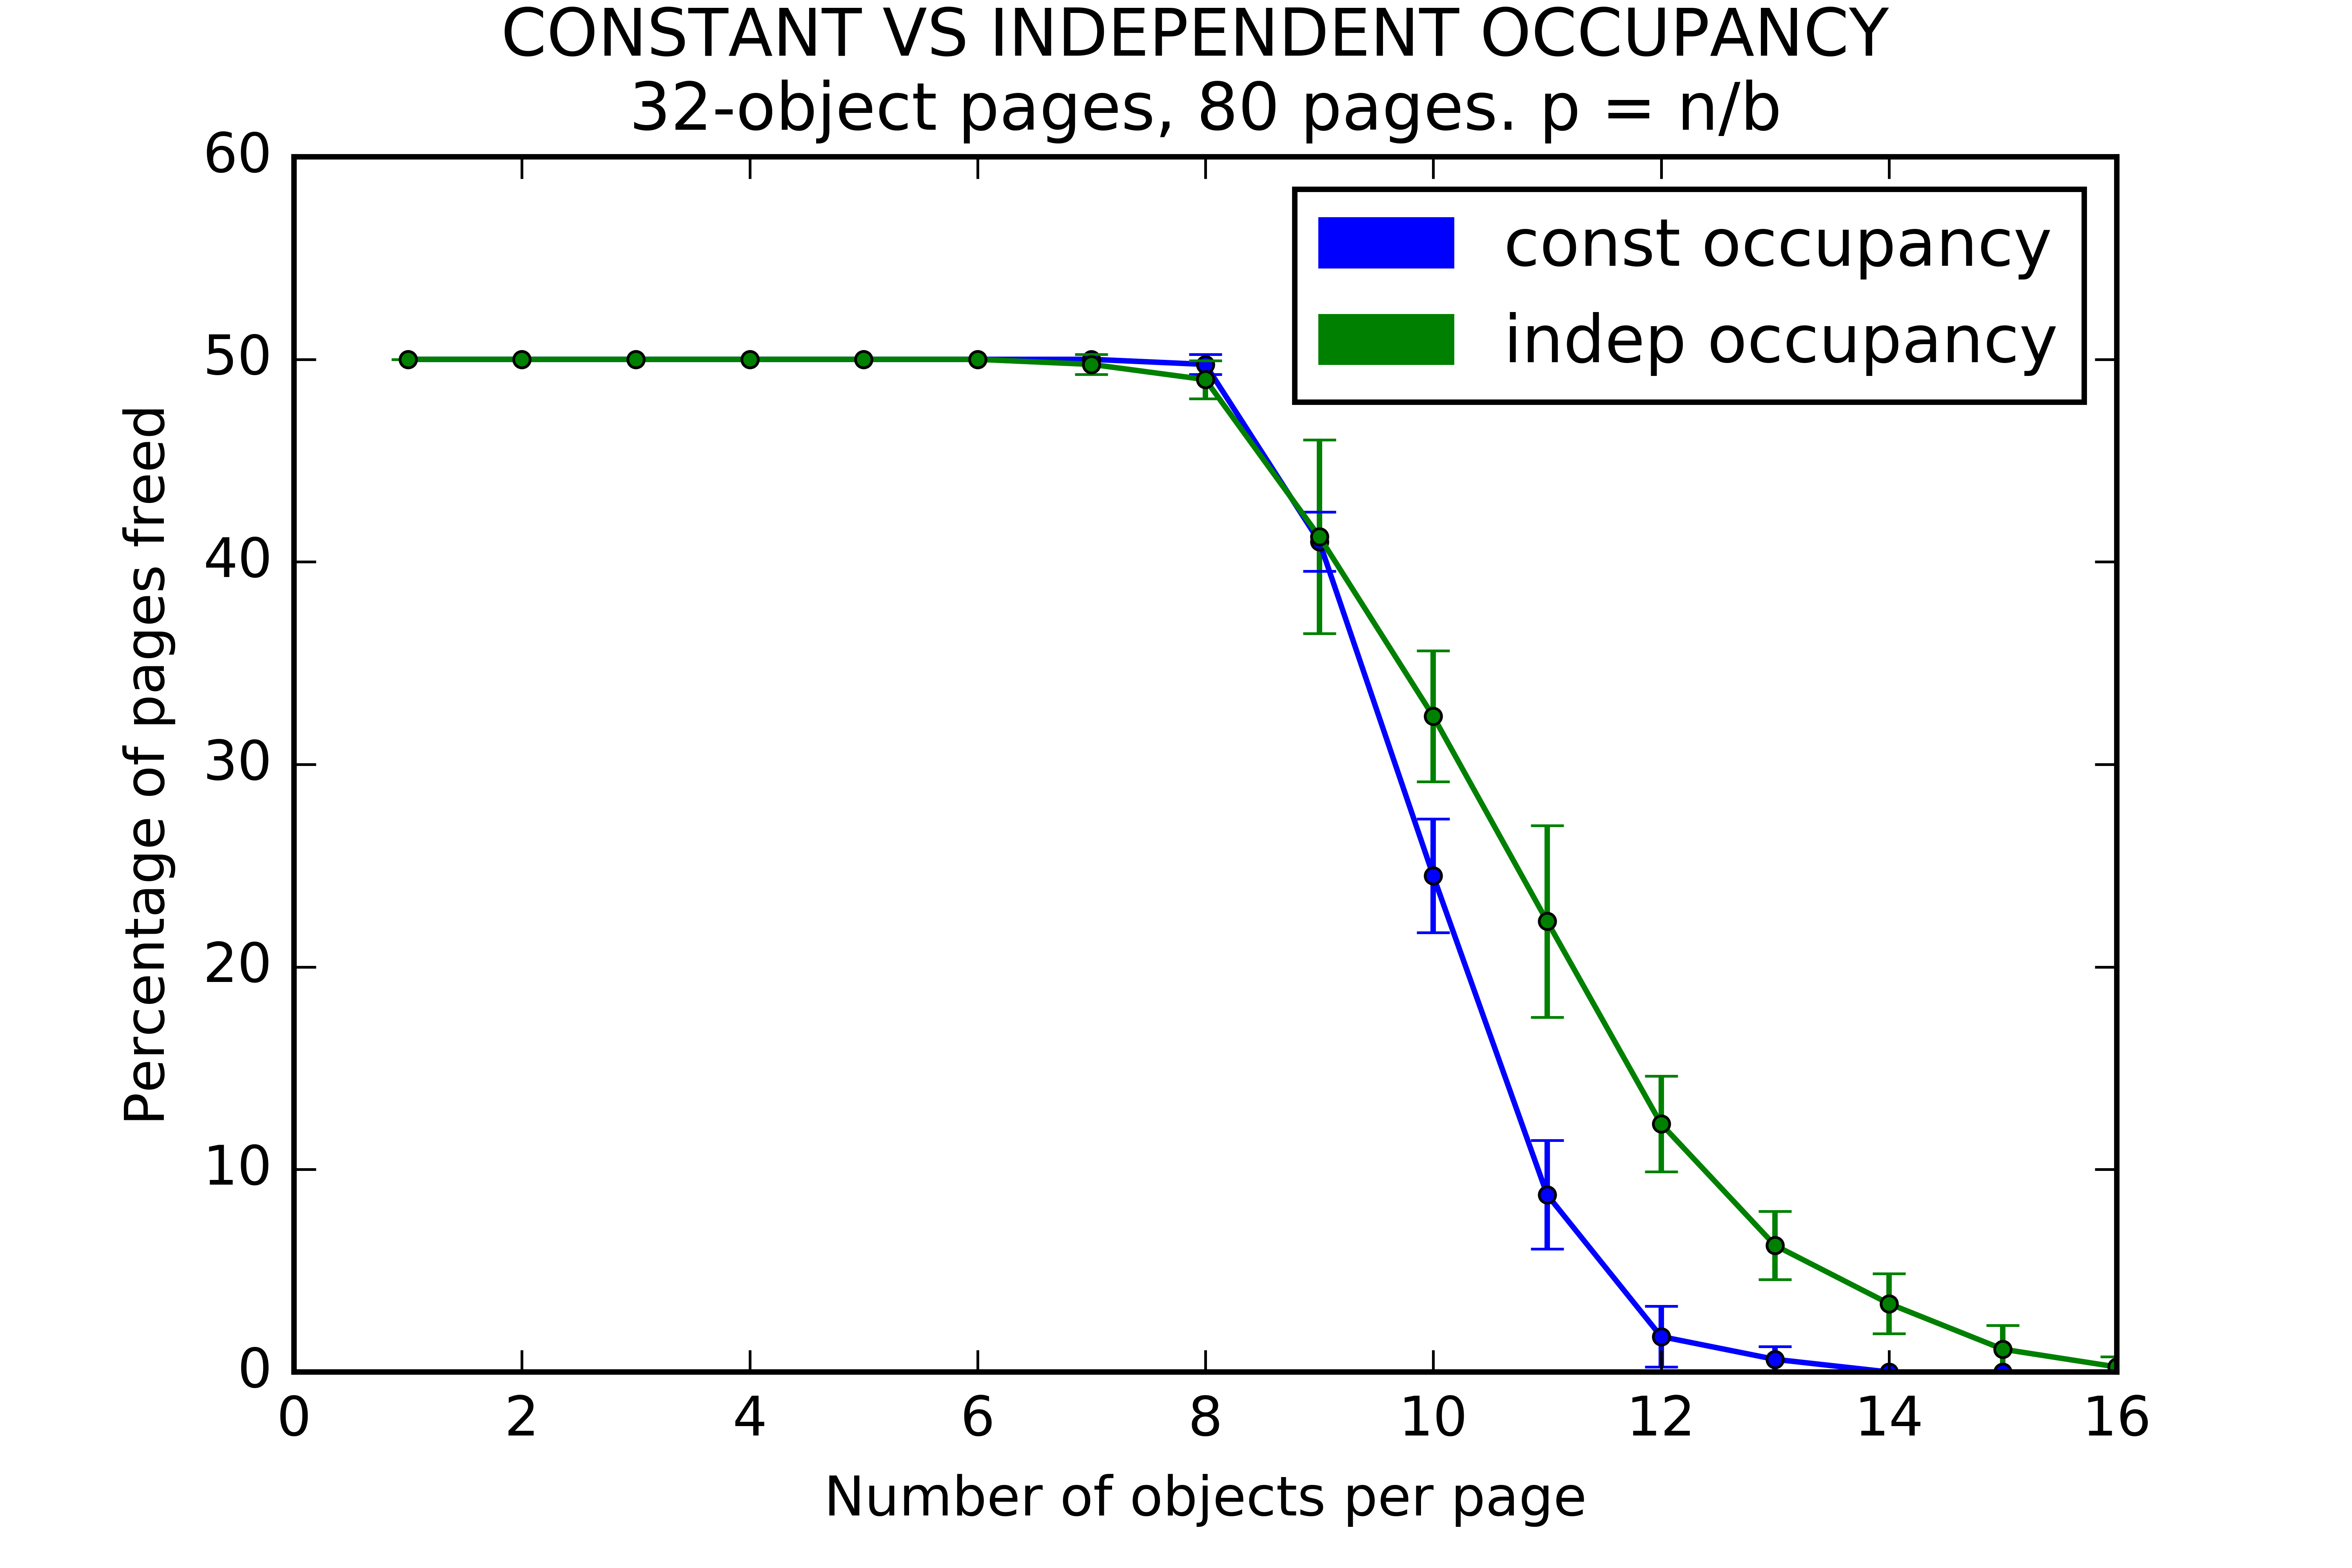
\includegraphics[scale = .5]{figures/constvindep_32,80.png}
\centering
\caption{Average values for max matching on randomly generated constant occupancy and independent bit graphs, $p = \frac{n}{b}$.  Ten graphs were generated for each occupancy.}
\end{figure}

Note that the maximum matching of the independent bit graphs are almost always equal to or larger than the max matching of the respective constant occupancy graphs.  Though we set $p$ so that both types of graphs will have (in expectation) the same occupancy, edges are more common in the indepedent bits model.  

\subsection{A new lower bound for Maximum Matching}
\subsection{A bound for general graphs}
McGregor et al. \cite{mcgregor16} show that:

\begin{theorem}
Define $W(G)$ to be a fractional matching on graph $G = (V,E)$ such that $$W = \sum_{(u,v) \in E} min(\frac{1}{deg(u)},\frac{1}{deg(v)})$$
Then $W\leq \frac{3}{2} M$ where $M$ is the cardinality of the maximum matching on $G$.
If $G$ is bipartite, then $W \leq M$.
\end{theorem}

For general graphs, $W$ is not always a lower bound on the maximum matching (hence the need for the $\frac{3}{2}$ factor).  For example, on a complete graph on three nodes, $W$ is $\frac{3}{2}$ while $M$ is 1.

\begin{figure}[h]
\includegraphics[scale = .7]{figures/triangle_matching.png}
\centering
\caption{W is not a lower bound for the maximum matching on a triangle.}
\end{figure}


While it is tight for this example, for larger non-bipartite graphs it seems like scaling $W$ down by $\frac{2}{3}$ is overkill.  For instance, for a complete graph on an odd number of nodes k, $W = {{k}\choose{2}} \frac{1}{k-1} = \frac{k}{2}$, while $M = \frac{k-1}{2}$.
The following theorem provides a tight lower bound for this example.

\begin{theorem}
Define $\W(G)$ to be a fractional matching on graph $G = (V,E)$ such that $$\W = \sum_{(u,v) \in E} min(\frac{1}{deg(u)+1},\frac{1}{deg(v)+1})$$
Then $\W \leq M$.
\end{theorem}
\begin{proof}
For $e = (u,v) \in G$, define $\W$$(e)=min(\frac{1}{deg(u)+1},\frac{1}{deg(v)+1})$.  Let $U$ be a node-induced subgraph of $G$.   Define $$\W(U) = \sum_{(u,v) \in U} \W(u,v)$$
As a corollary of Edmonds Matching Polytope Theorem, a fractional matching on a graph is a lower bound for the maximum matching if for any node-induced subgraph $U$ of $G$ of odd size, $\W(U) \leq \frac{t-1}{2}$.


\begin{align*} 
\W(U) &= \sum_{(u,v) \in U} min(\frac{1}{deg(u)+1},\frac{1}{deg(v)+1})\\
& \leq \sum_{(u,v) \in U}\frac{1}{2}(\frac{1}{deg(u)+1}+\frac{1}{deg(v)+1})\\
&\leq \sum_{(u,v) \in U}\frac{1}{2}(\frac{1}{deg_U(u)+1}+\frac{1}{deg_U(v)+1})\\
&= \frac{1}{2} \sum_{u \in U} \frac{deg_U(u)}{deg_U(u)+1} \leq  \frac{1}{2} (\frac{t-1}{t}) t = \frac{t-1}{2}\\
\end{align*}
The second line follows from the fact that the minimum of two quantities is bounded above by their average.  The third line follows from the fact that the degree of any node in a subgraph is bounded above by its degree in the original graph.  The fourth line follows from summing over nodes instead of edges, and then reasoning that in the worst case U is a clique and thus $deg_U(u) = t-1$ for all u $u$. 
\end{proof}

\subsection{Improvements to $\W$}
In some cases $\W$ is too conservative; it assigns little weight to edges which it could safely have assigned much more.  For example, if $e$ is isolated (meaning its endpoints have degree 1), $\W(e) = \frac{1}{2}$.  However, it is always safe to assign weight 1 to $e$, since $M(G-e) = M(G)-1.\footnote{Here we use M(G) to denote the cardinality of the maximum matching on G.}$  If we modified our rule for $\W$ so that for any edge $e= (u,v)$ s.t. $deg(u)=deg(v) = 1$ we assigned weight $ min(\frac{1}{deg(u)},\frac{1}{deg(v)})$ instead of $ min(\frac{1}{deg(u)+1},\frac{1}{deg(v)+1})$, we would always assign weight 1 to isolated edges.

At this point it is natural to ask whether we can remove the $+1$s from the denominator for other edges.  We cannot of course do so for $deg(u) = deg(v) = k >1, k \in 2\mathbb{Z}$ since for a clique on k+1 nodes this rule would result in total weight $\frac{k+1}{2}$.\\

Below we prove several rules of this form.  For each rule we specify values of $deg(u)$ and $deg(v)$ for which the $+1$ can be removed from the denominator of the edge weight.  First we restate the claim that isolated edges may safely be assigned weight 1.

\begin{lemma}
Define $\W(G)$ as follows:\\
For each $(u,v) \in G$,\\
if $deg(u) = deg(v) = 1$, $\W(u,v) =  min(\frac{1}{deg(u)},\frac{1}{deg(v)})$.\\
else $\W(u,v) =  min(\frac{1}{deg(u)+1},\frac{1}{deg(v)+1})$.

Then $\W(G) \leq M(G)$.

\end{lemma}
\begin{proof}
Already proven above.
\end{proof}

Next we will amend $\W$ to include the following rule: when one endpoint has degree 1 and the other has degree k, assign weight $\frac{1}{k}$.

\begin{lemma}
Define $\W(G)$ as follows:\\
For each $(u,v) \in G$,\\
if $deg(u) = 1$, $\W(u,v) =  min(\frac{1}{deg(u)},\frac{1}{deg(v)})$.\\
else $\W(u,v) =  min(\frac{1}{deg(u)+1},\frac{1}{deg(v)+1})$.

Then $\W(G) \leq M(G)$.
\end{lemma}
\begin{proof}
We have proven that $W(U)\leq \frac{t-1}{2}$ on any odd-size subgraph $U$, $|U| = t$.  Define subsets $U_1$ and $U_2$ of $U$ such that $U_1 \cup U_2 = U$.  $U_1$ is the set of all nodes in $U$ of degree 1 and all nodes in $U$ adjacent to a node of degree 1, and $U_2$ is the set of all other nodes in $U$.  Let $G(U_2)$ denote the subgraph of $U$ induced by $U_2$, and let $|U_1| = x$ where x is even.  Then $W(G(U_2)) = \W(G(U_2)) \leq \frac{t-x-1}{2}$.  So to complete our proof we must show that all remaining edges (call them $E'$) have total weight $\leq \frac{x}{2}$.

Assume WLOG that there are no isolated edges in $G$ (if there are, we can group them with $G(U_2)$ and retain the $\frac{t-x-1}{2}$ bound).

\begin{align*}
\W(E') & \leq \frac{1}{2} \sum_{u,v \in E'} (\frac{1}{deg(u)}+\frac{1}{deg(v)})\\
& = \mathlarger{\sum_k} \Big(\sum_{v \in U_1, deg(v) = k} \frac{\delta}{k} + \frac{k-\delta}{2(k+1)}\Big)
\end{align*}
where $\delta$ denotes the number of degree 1 nodes adjacent to $v$.\\
Let $f(\delta) = \frac{\delta}{k} + \frac{k-\delta}{2(k+1)}$.  We are interested in finding the maximum value $\frac{f(\delta)}{\delta+1}$ can take on; if it can never take a value greater than $\frac{1}{2}$ then $\W(E')$ cannot be greater than $\frac{x}{2}$.

$$\frac{\partial\frac{f(\delta)}{\delta+1}}{\partial \delta} = \frac{2-k}{2k(\delta+1)^2}$$

which is always negative for $k \geq 2$.  Thus $\frac{f(\delta)}{\delta+1}$ is maximized at $\delta = 0$, so  $\frac{f(\delta)}{\delta+1} \leq \frac{k}{2(k+1)} < \frac{1}{2}.$

There is one final detail we have not considered: $x$ might be odd.  In this case, $|U_2|$ is even thus we can't appeal to Theorem 3 to say that $\W(G(U_2)) \leq \frac{t-x-1}{2}$.  However, we can simply remove one node $\node'$ from $U_2$; the resulting odd-size subgraph has weight at most $\frac{t-x-2}{2}$.  Since $\W$ is a valid fractional matching, the weight assigned to all edges adjacent to $\node'$ cannot exceed 1, thus we can say that $\W(G(U_2)) \leq \frac{t-x}{2}$.  Now we must show that $\W(E') \leq \frac{x-1}{2}$.

We have shown that the edge weight per node in $U_1$ cannot exceed $\frac{1}{2}$.  $\W(E')$ is minimized when there is exactly 1 node of degree 1, with a degree k neighbor. In this case, the only edge in $E'$ will be assigned weight $\frac{k}{2(k+1)}<\frac{1}{2}$.  Thus, $\W(E') \leq \frac{1}{2} + \frac{x-2}{2} = \frac{x-1}{2}$ and the lemma is proven.  
\end{proof}

Finally, we further amend $\W$ to include the following rule:  when one endpoint has degree 2 and the other degree 3, assign weight $\frac{1}{3}$.

\begin{lemma}
Define $\W(G)$ as follows:\\
For each $(u,v) \in G$,\\
if $deg(u) = 1$, or if $deg(u) = 2$ and $deg(v) = 3$, $\W(u,v) =  min(\frac{1}{deg(u)},\frac{1}{deg(v)})$.\\
else $\W(u,v) =  min(\frac{1}{deg(u)+1},\frac{1}{deg(v)+1})$.

Then $\W(G) \leq M(G)$.
\end{lemma}
\begin{proof}
Omitted for space.
\end{proof}

One might wonder whether a more general rule can be proven.  So far the only counterexamples we have presented to W being a lower bound are complete graphs of odd size.  We might try to avoid these failed cases by defining $\W$ so that we include the $+1$ in the denominator only when $deg(u) = deg(v) \neq 1$.  In this case, the total weight on a odd-size complete graph is exactly $\frac{t-1}{2}$.

However, this rule gives weight $3(\frac{1}{5}) + 6(\frac{1}{4})$ for a complete graph on five nodes with one edge removed, which is larger than the $\frac{5}{2}$ limit from Edmond's theorem.  So this rule doesn't produce a valid lower bound for maximum matching. 

Currently we are hoping to determine whether the following conjecture is true:
\begin{conjecture}
Define $\W(G)$ as follows:\\
For each $(u,v) \in G$,\\
if $deg(u) = deg(v)$, or if $deg(u) = k$ and $deg(v) = k+1$,$\W(u,v) =  min(\frac{1}{deg(u)+1},\frac{1}{deg(v)+1})$.\\
else $\W(u,v) =  min(\frac{1}{deg(u)},\frac{1}{deg(v)})$.

Then $\W(G) \leq M(G)$.
\end{conjecture}